\def\year{2021}\relax
%File: formatting-instructions-latex-2021.tex
%release 2021.1
\documentclass[letterpaper]{article} % DO NOT CHANGE THIS
\usepackage{aaai21}  % DO NOT CHANGE THIS
\usepackage{times}  % DO NOT CHANGE THIS
\usepackage{helvet} % DO NOT CHANGE THIS
\usepackage{courier}  % DO NOT CHANGE THIS
\usepackage[hyphens]{url}  % DO NOT CHANGE THIS
\usepackage{graphicx} % DO NOT CHANGE THIS
\urlstyle{rm} % DO NOT CHANGE THIS
\def\UrlFont{\rm}  % DO NOT CHANGE THIS
\usepackage{natbib}  % DO NOT CHANGE THIS AND DO NOT ADD ANY OPTIONS TO IT
\usepackage{caption} % DO NOT CHANGE THIS AND DO NOT ADD ANY OPTIONS TO IT
\frenchspacing  % DO NOT CHANGE THIS
\setlength{\pdfpagewidth}{8.5in}  % DO NOT CHANGE THIS
\setlength{\pdfpageheight}{11in}  % DO NOT CHANGE THIS
%\nocopyright
%PDF Info Is REQUIRED.
% For /Author, add all authors within the parentheses, separated by commas. No accents or commands.
% For /Title, add Title in Mixed Case. No accents or commands. Retain the parentheses.
% /Title ()
% Put your actual complete title (no codes, scripts, shortcuts, or LaTeX commands) within the parentheses in mixed case
% Leave the space between \Title and the beginning parenthesis alone
% /Author ()
% Put your actual complete list of authors (no codes, scripts, shortcuts, or LaTeX commands) within the parentheses in mixed case.
% Each author should be only by a comma. If the name contains accents, remove them. If there are any LaTeX commands,
% remove them.

% DISALLOWED PACKAGES
% \usepackage{authblk} -- This package is specifically forbidden
% \usepackage{balance} -- This package is specifically forbidden
% \usepackage{color (if used in text)
% \usepackage{CJK} -- This package is specifically forbidden
% \usepackage{float} -- This package is specifically forbidden
% \usepackage{flushend} -- This package is specifically forbidden
% \usepackage{fontenc} -- This package is specifically forbidden
% \usepackage{fullpage} -- This package is specifically forbidden
% \usepackage{geometry} -- This package is specifically forbidden
% \usepackage{grffile} -- This package is specifically forbidden
% \usepackage{hyperref} -- This package is specifically forbidden
% \usepackage{navigator} -- This package is specifically forbidden
% (or any other package that embeds links such as navigator or hyperref)
% \indentfirst} -- This package is specifically forbidden
% \layout} -- This package is specifically forbidden
% \multicol} -- This package is specifically forbidden
% \nameref} -- This package is specifically forbidden
% \usepackage{savetrees} -- This package is specifically forbidden
% \usepackage{setspace} -- This package is specifically forbidden
% \usepackage{stfloats} -- This package is specifically forbidden
% \usepackage{tabu} -- This package is specifically forbidden
% \usepackage{titlesec} -- This package is specifically forbidden
% \usepackage{tocbibind} -- This package is specifically forbidden
% \usepackage{ulem} -- This package is specifically forbidden
% \usepackage{wrapfig} -- This package is specifically forbidden
% DISALLOWED COMMANDS
% \nocopyright -- Your paper will not be published if you use this command
% \addtolength -- This command may not be used
% \balance -- This command may not be used
% \baselinestretch -- Your paper will not be published if you use this command
% \clearpage -- No page breaks of any kind may be used for the final version of your paper
% \columnsep -- This command may not be used
% \newpage -- No page breaks of any kind may be used for the final version of your paper
% \pagebreak -- No page breaks of any kind may be used for the final version of your paperr
% \pagestyle -- This command may not be used
% \tiny -- This is not an acceptable font size.
% \vspace{- -- No negative value may be used in proximity of a caption, figure, table, section, subsection, subsubsection, or reference
% \vskip{- -- No negative value may be used to alter spacing above or below a caption, figure, table, section, subsection, subsubsection, or reference

\setcounter{secnumdepth}{2} %May be changed to 1 or 2 if section numbers are desired.

% The file aaai21.sty is the style file for AAAI Press
% proceedings, working notes, and technical reports.
%
\title{Intelligent Recommendations for Citizen Science}
%Your title must be in mixed case, not sentence case.
% That means all verbs (including short verbs like be, is, using,and go),
% nouns, adverbs, adjectives should be capitalized, including both words in hyphenated terms, while
% articles, conjunctions, and prepositions are lower case unless they
% directly follow a colon or long dash

\author{
 % Authors
  %Na'ama Dayan,\textsuperscript{\rm 1}
    Daniel Ben Zaken, \textsuperscript{\rm 1}
    Kobi Gal, \textsuperscript{\rm 1,3}
    Guy Shani \textsuperscript{\rm 1}
    Avi Segal \textsuperscript{\rm 1} and
    Darlene Cavalier. \textsuperscript{\rm 2}
    \\
    \\
}
\affiliations{
    %Afiliations
    \textsuperscript{\rm 1}Ben-Gurion University,
        \textsuperscript{\rm 2}  Arizona State University, \\
     \textsuperscript{\rm 3} University of Edinburgh \\
    benzaked@post.bgu.ac.il,

  \{kobig, shanigu, avise\}@bgu.ac.il, \\
    darlene@scistarter.com
 %   firstAuthor@affiliation1.com, secondAuthor@affilation2.com,
    }


\newcount\Comments  % 0 suppresses notes to selves in text
\Comments=0

\usepackage{xcolor}
% \definecolor{green}{rgb}{0,1,0}
\newcommand{\kibitz}[2]{\ifnum\Comments=1{\textcolor{#1}{#2}}\fi}
\newcommand{\nh}[1]{\kibitz{blue}{[NH:#1]}}
\newcommand{\kg}[1]{\kibitz{red}{[KG:#1]}}
\newcommand{\as}[1]{\kibitz{ orange}{[AS:#1]}}
\newcommand{\bg}[1]{\kibitz{green}{[BG:#1]}}
 \begin{document}

\maketitle
\begin{abstract}
%We report on the use of AI based recommendation tools to match thousands of volunteers with suitable Citizen Science projects.
Citizen science refers to scientific research that is carried out by volunteers, often in collaboration with professional scientists.
The spread of the internet has allowed volunteers to contribute to citizen science projects in  dramatically new ways while creating scientific value and gaining pedagogical and social benefits.
%For example, SciStarter, our partners in the project, is an online portal that offers more than  3,000 affiliate projects and recruits volunteers through media and other organizations, bringing citizen science to people.
Given the sheer size of available projects, finding the right project, which best suits the user preferences and capabilities, has become a major challenge and is essential for keeping volunteers motivated and active contributors.
We address this challenge by developing a system for personalizing  project recommendations which was fully deployed in  the wild.
We adapted several recommendation algorithms to the citizen science domain from the literature based on memory-based and model-based collaborative filtering approaches.  The algorithms were trained on historical data of users' interactions in the SciStarter platform - a leading citizen science site -
as well as their contributions to different projects.
The trained algorithms were evaluated in SciStarter and involved hundreds of users who were  provided with personalized recommendations for  new  projects they had not contributed to before. %Volunteers were randomly divided into different cohorts, which varied the recommendation algorithm that was used to generate suggested projects.
The results show that using the new recommendation system  led people to  increased participation in new SciStarter projects when compared to   groups that were recommended projects using non-personalized
 recommendation approaches,
and compared to behavior before recommendations.   In particular, the group of volunteers receiving recommendations created by an SVD algorithm (matrix factorization) exhibited the highest levels of contributions to new projects, when compared to the other cohorts.
A follow-up survey conducted with the SciStarter
community confirmed that users felt that the recommendations  matched their personal interests and goals.
Based on these results, our recommendation system is now fully integrated into the SciStarter  portal, positively affecting hundreds of users each week, and  leading to social and educational benefits.
%The research has transformed how SciStarter helps projects recruit and support participants and better respond to their needs.
%This is the first study using AI based recommendation tools in large scale citizen science platforms.

%This work lays the foundation to enhance participants’ motivation and learning in citizen science by aligning interests with projects through AI recommendation tools.
\end{abstract}

% * <john.hammersley@gmail.com> 2015-02-09T12:07:31.197Z:
%
%  Click the title above to edit the author information and abstract
%
\section{Introduction}

Citizen science engages people in scientific research  by collecting, categorizing, transcribing, or analyzing scientific data \cite{bonney2009citizen,funk2017science,brossard2005scientific}.
 These platforms
 offer thousands of different projects which rely on the contributions of volunteers to extend
 scientific knowledge.

    Citizen science brings   significant scientific, pedagogical and social benefits. It provides new ways for the public to
   contribute to scientific research: Volunteers
   can share and contribute to data monitoring and collection programs. Community-based groups can generate ideas and engage with scientists for advice, leadership, and program coordination~\cite{silvertown2009new,bonney2014next,ryan2018role}. Citizen science can be used as an educational tool, allowing students, educators and scientists to  network and promote new ideas to advance our understanding of the world~\cite{vitone2016school}. Lastly, citizen science contributes to social inclusion by increasingly engaging volunteers from underrepresented and marginalised communities~\cite{haywood2014education,sorensen2019reflecting}.


      SciStarter (\url{scistarter.org}) is  an online citizen science hub  which aggregates over
      3,000 projects that are imported through partnerships with federal governments, NGOs, and universities. It is the world’s largest catalogue of citizen science projects.  Projects span different topics, age groups, location, etc. As of July 2020, SciStarter had  82,014 registered users   from diverse age groups, socio-economic and educational backgrounds. Hundreds of the projects use SciStarter supported APIs to collect data from volunteers, who can track their participation  across projects in their SciStarter dashboard. SciStarter maintains
      an active forum where volunteers and researchers can communicate directly. In addition to its scientific contribution, SciStarter also plays an important educational and social role. It collaborates with
     different institutions (schools, universities, libraries, museums, Girl Scouts, Discover magazine, and more)  to customize citizen science pathways, and participates in
      organized events such as ``Citizen Science Month" that promote hundreds of projects all over the world.

      Volunteers visit SciStarter in order to discover new projects and keep up to date with   community events.
       Examples of popular projects on the SciStarter platform include iNaturalist~\footnote{\url{https://scistarter.org/seek-by-inaturalist}} in which users map and share observations of biodiversity across the globe; CoCoRaHS~\footnote{https://scistarter.org/cocorahs-rain-hail-snow-network}, where volunteers share daily readings of precipitation; and StallCatchers~\footnote{https://scistarter.org/stall-catchers-by-eyesonalz}, where volunteers identify vessels in the brain as flowing or stalled.
      Figure \ref{fig:ui} shows the  SciStarter main page window, including a search engine to locate projects, and a featured project that is hand-selected
      by the SciStarter admins.

      %These features enable SciStarter's partners (libraries, schools, museums, Girl Scouts and more) to catalyze customized citizen science pathways and track and support the progress of their communities through SciStarter.
      %SciStarter also supports researchers in managing projects, including best practices for engaging participant partners.


% % Examples of popular projects on SciStarter include
% % iNaturalist in which users map and share observations of biodiversity across the globe;
% %  CoCoRaHS, in which volunteers share  daily readings of precipitation;
% %  and StallCatchers, in which volunteers  identify vessels in the brain as flowing or stalled.
% SciStarter is a citizen science platform, which offers over 3000 projects to more than 65000 registered users.
 %Projects can be taken either online or at a specific physical region.

\begin{figure}[t]
\centering
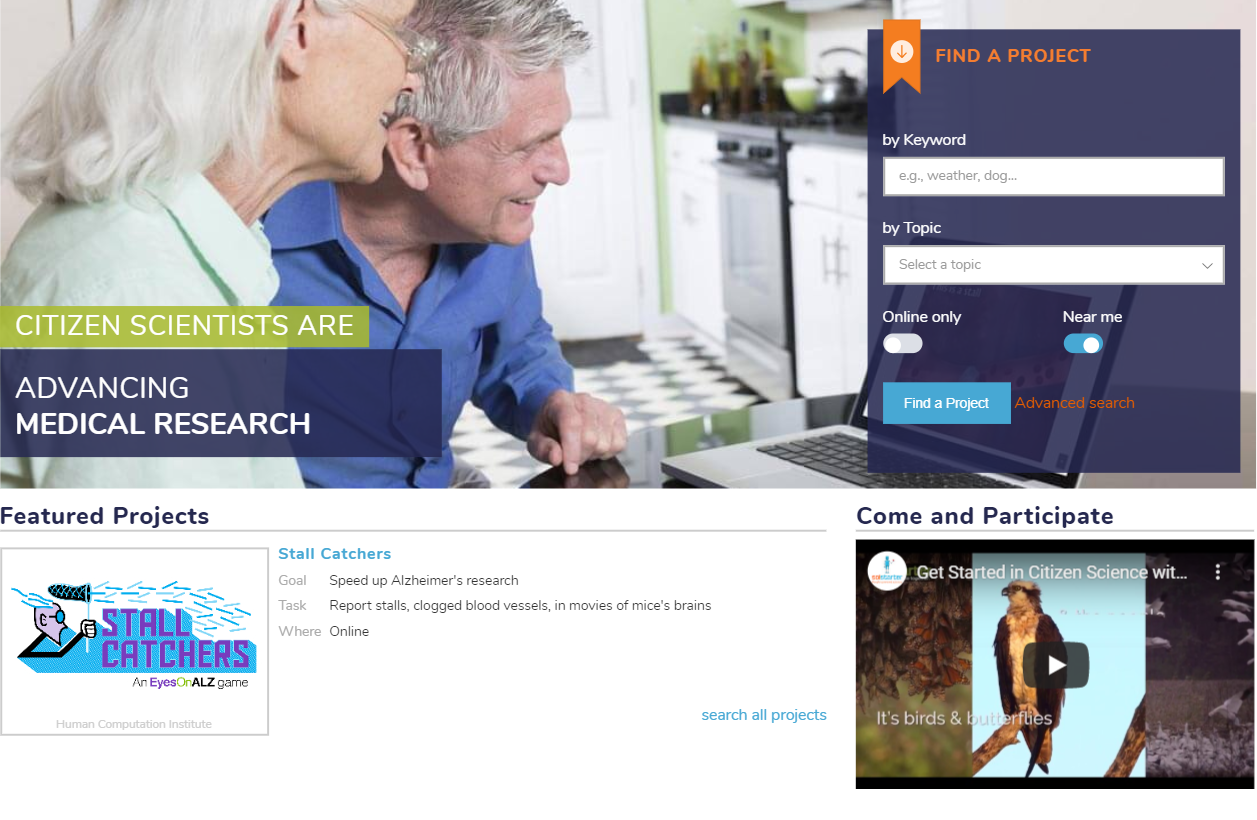
\includegraphics[width=8cm]{Figs/SciStarterUI.PNG}
\caption{SciStarter User Interface}
\label{fig:ui}
\end{figure}



 SciStarter is one of several large scale citizen science portals, (such as Zooniverse (https://www.zooniverse.org/), CitSci.org, and
Anecdata.org)
 that host between hundreds to thousands of different   projects and  connect volunteers, researchers and educators. On the one hand,
 the breadth and size of these portals provide an abundance of opportunities  for volunteers to discover and contribute to new projects.
  There is evidence showing that   motivated volunteers can provide quality contributions
  for several citizen science projects, increasing their social value in addition to their scientific contributions~\cite{larson2020diverse}.
  On the   other hand, the vast majority of citizen science volunteers perform tasks regularly in very few projects~\cite{ponciano2019characterising}. To illustrate,
    Figure~\ref{fig:pinp} shows a histogram
  of the number of projects that users contributed to on the site between 2017 and 2019. As shown by the figure, the   majority of active users in the SciStarter portal do not contribute to more than a single project.  A similar pattern of contributions was observed in the
  Zooniverse citizen science portal~\cite{segal2018optimizing}.

To help users discover new projects, SciStarter employs  a search engine  where users can find projects  according to topics (e.g., Archaeology), activities (e.g., can be done online), location (e.g., at a science center or zoo) or age groups.
However, recommending projects based on this tool has not been successful.  Our analysis shows that about 80\% of users do not use the search tool. In addition, data also shows that when users \emph{do} use the search engine, most of them do not   visit the projects that are outputted by the tool for their selection. Clearly, a more sophisticated approach is needed in this domain to match people with the right projects.
%For example, when querying outdoor projects, the search engine
%recommends the  CoCoRaHS project and Globe at Night, in which volunteers measure and submit their night sky brightness observations.    But  data shows that people who join CoCoRaHS are more likely to join Stall Catchers, an indoor, online project to accelerate Alzheimer’s research.\as{this eexample not clear. Maybe remove}
%Most volunteers  rarely come back to the SciStarter portal   once they have converged on a project they contribute to regularly,
  %which further exasperates the difficulty of providing them with beneficial  recommendations.

% Yet,

%  ** talk about only trying one project **

%   Ponciano and Pereira~\shortcite{ponciano2019characterising} characterized volunteers' task execution patterns across projects and showed that volunteers tend to explore multiple projects in citizen science platforms, but they


\begin{figure}[t]
\centering
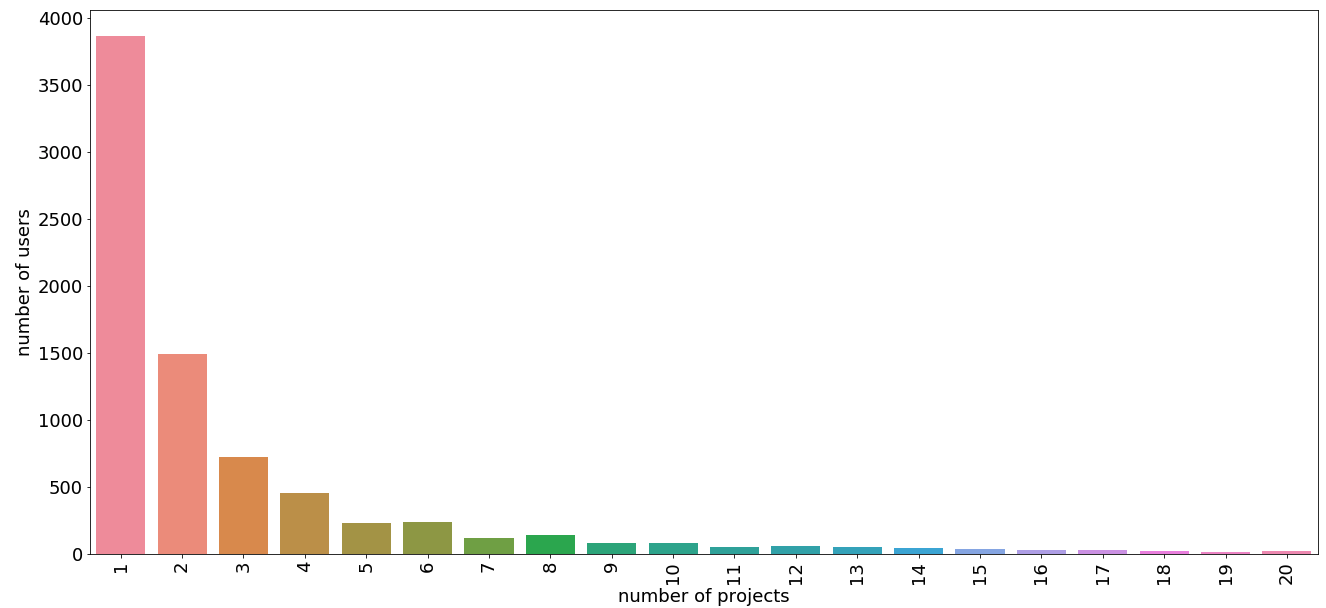
\includegraphics[width=8cm]{Figs/participation histogram.png}
\caption{Distribution of user participation in SciStarter projects
}
\label{fig:pinp}
\end{figure}


%Clearly,
 % matching users with the projects that are most suitable for their preferences
 % is a real challenge.
  %This hurts science, too, as the collective output of the projects does not meet its potential.

%SciStarter employs  a search engine that uses topics, activities, location and demographics  to assign project recommendations. In the past,


% \begin{figure}[h]
% \centering
% 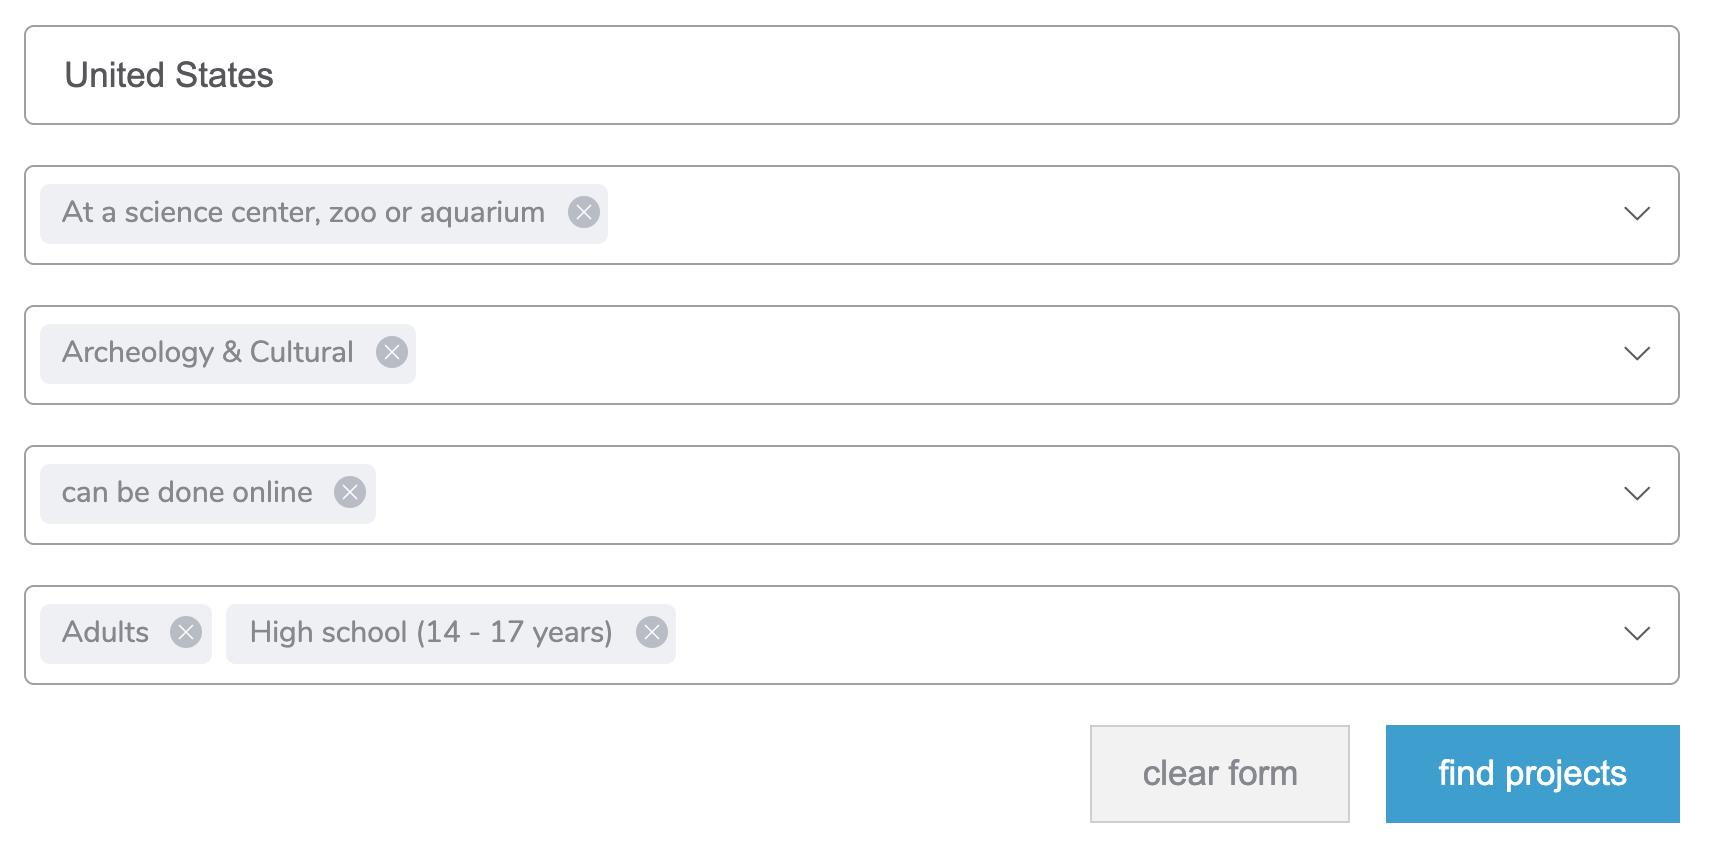
\includegraphics[width=8cm]{Figs/searchScreen.png}
% \caption{Screenshot of existing search tool showing various  criteria}
% \label{fig:search}
% \end{figure}
% %  Most citizen science volunteers  make only a few contributions to one or two projects and seldom return to the
%  site~\cite{ricci2015recommender, burgess2017science}. This hurts science, too, as the collective output of the projects does not meet its potential. Thus, a universal challenge for citizen science, “is attracting and retaining enough participants to make achievement of project goals possible.”~\cite{crowston2013motivation}.


 In this paper, we take an AI approach towards solving the
 recommendation problem in citizen science: how to match volunteers
 with new project recommendations in order to increase the
 number of activities that volunteers contribute to new projects on
 the SciStarter ecosystem.
  We match individual volunteers with new projects based on the  past history of their interactions on the site~\cite{dwivedi2017recommender,amatriain2013big}.

  According to a report from the National Academies of Sciences, Engineering, and Medicine~\cite{national2018learning}, citizen scientists’ motivations are ``strongly affected by personal interests,” and participants who engage in citizen science over a long period of time ``have successive opportunities to broaden and deepen their involvement.”
  %Thus,   sustained engagement through the use of intelligent recommendations can improve data quality and scientific outcomes for the projects and the public.
 Thus our  hypothesis was  twofold. First, that
 personalizing recommendations  to volunteers
 will increase their engagement in  SciStarter and improve scientific outcomes,   as measured by
 the number of projects that they contribute to, after being presented with  recommendations, as well as  the extent of their contributions to these projects.
 Second, that users will be satisfied with the recommendation tool and continue to be motivated
 contributors to SciStarter.


  Recommendation systems have been used in other  domains, such as e-commerce, news, and  social media \cite{itmazi2006recommendation,fleder2007recommender,kleinerman2020supporting}.  However,
  the nature of interaction in citizen science is fundamentally different  than these domains. In citizen science,
 volunteers  are actively encouraged to contribute their time and effort to solve scientific problems~\cite{cohn2008citizen}.
 Most citizen scientists contribute to  few projects, compared to participants in online marketplaces and news sites who consume multiple items (e.g., movie recommendations).
 %This lack of diversity in
 %users' interactions challenges
 %Collaborative Filtering    algorithms that  are based on aggregating histories of user interactions on the site.
 Thus solving the recommendation problem for citizen science can be considered a contribution from both scientific and social perspectives.

%  For example,  movie goers will often see several  movies, and see each movie once,  while  citizen scientists mostly contribute to a single project, and make several contributions to this project. Getting users
%  T

 %Compared to traditional
 %Compared to clicking on an advertisement or a product, as is the case for e-commerce and news sites, considerable more cognitive  effort is required
%  %from a citizen science volunteer.
%  We match individual volunteers with new projects based on the  past history of their interactions on the site~\cite{dwivedi2017recommender,amatriain2013big}.

 To address these challenges, we adapted  different recommendation algorithms to the citizen science domain. Each algorithm matches a user profile and the user's past history of interactions and outputs a ranking of the most relevant $n$  projects   for the user, in decreasing order of relevance.
%The input to each algorithms  consists of data representing users' interactions with      projects (e.g.,   joining or contributing to a project),  and users' interactions   on the  SciStarter portal, (e.g., searching for or clicking on a project link).  The output
%of each algorithm  is a function from user profile to a  ranking of the   projects in order of
%inferred relevance for the  user.

% We measured two types of user interactions, which were taken as the input to the algorithms: (1) Interactions with projects: data generated as a result of users’ activities with projects, e.g joining a project, making a contribution to a project or participating in a project. (2) Interactions on SciStarter portal, such as clickling on a project link, or searching for a specific project.


% We delivered recommendations to sign-in users only, and users could choose to opt-out from receiving recommendations.

We conducted a randomized controlled study, in which hundreds of registered SciStarter users were randomly divided into cohorts,
and
assigned recommendations using different approaches.
The first approach personalized projects to participants by  using  memory-based collaborative filtering algorithms  (recommending projects to users based on user or item similarity),  and matrix factorization algorithms (predicting the
relevance of a new  project to a user based on learned latent spaces).
These algorithms were compared to two non-personalized algorithms:
the first algorithm recommended the most popular projects to users, and the second algorithm
recommended  promoted    projects that were manually determined by  SciStarter admins at regular intervals (e.g., promoting a biology based project for Science Day).

The results show that  people receiving the personalized recommendations  were more likely  to contribute to new projects that they had never tried before and participated more often in
these projects  when compared to participants who received non-personalized recommendations, or compared to behavior before
the recommendations. In particular, the cohort of participants receiving recommendations created by the matrix factorization algorithm exhibited the highest levels of contributions to the recommended projects, when compared to the other personalized groups.

In a  follow-up survey conducted with the SciStarter community, volunteers
expressed high satisfaction with the recommendation tool, providing further support for its positive impact on engagement.
Based on the positive results, our recommendation system is now fully integrated with SciStarter,  providing
recommendations to hundreds of users each day, significantly increasing
the number of contributions in new projects by volunteers.  This is the first study using AI based recommendation algorithms in a large scale  citizen science platform.

\section{Related Work}
 This research relates to past work in using AI to increase participants' motivation in  citizen science research as well as work in applying recommendation systems in real world settings. We list relevant work in each of these two areas.

Active  participation  in citizen science projects through the internet is growing  fast \cite{nov2014scientists,Irwin2018NoPN}. Yet, most participants   participating in citizen science projects perform only a few tasks each before leaving the system \cite{rotman2012dynamic}. For example,  less than 10\% of all users   contribute to more than 10 projects in the SciStarter portal.
This reflects a general trend in  volunteer-based crowdsourcing, whereby  the majority of participants carry out only a few tasks~\cite{segal2016intervention,segal2015improving}.


 Ponciano et al. \shortcite{ponciano2019characterising}   showed that although volunteers tend to explore multiple projects in citizen science platforms,  they perform tasks regularly in just a few of them. They   also showed that volunteers recruited from other projects on the platform tend to get more engaged than those recruited outside the platform. This finding motivated our approach
to recommend suitable projects for  SciStarter .

Several works  have studied the motivations of participants  in citizen science.
Kragh et al. \shortcite{kragh2016motivations} showed that participants in citizen science projects are motivated by personal interest and a desire to learn something new, as well as their desire to volunteer and contribute to science.
% Nov et al. \cite{nov2014scientists}  showed that quantity of contribution in citizen science projects is mostly determined by the user interest in the project   while quality of contribution depends more on understanding the task as well as the user's reputation.
Raddic et al. \shortcite{raddick2009galaxy}  claimed that citizen scientists  mostly exhibit interest in a single  topic, such as astronomy and zoology. The  user survey  we
conducted on SciStarter reveals participants'  interests to be more diverse and span multiple projects.

Other works have designed interventions for the purpose of  increasing  participants' engagement in citizen science.
Segal et al. \shortcite{segal2018optimizing,segal2016intervention}  used AI planning to  personalize  motivational message
policies which significantly increase users’ contributions.
Laut et al. \shortcite{laut2017increasing}  showed that participants’ contributions can be enhanced through the presence of virtual peers.



Several approaches have used recommendation algorithms to increase participants'  engagement   in education and social media settings. Labarthe et al. \shortcite{labarthe2016does} recommended educational content
for students in Massive Open Online Courses (MOOCs)   based on student profiles and their online activities.    Dwivedi et al. \shortcite{dwivedi2017recommender} used collaborative filtering to  recommended  online courses to students based on their past grades.  Freyne et al. \shortcite{freyne2009increasing} generated  recommendations to users during sign-up
to social network sites by leveraging aggregated external data from other
social media sites.
In contrast to these systems, users' profiles in SciStarter do not contain
information relating to their project  preferences, and we do not have access to their
task performance correctness in the projects.
% This paper showed that users who interacted with the recommendation system increased their chance to finish the MOOC by 270\%, compared to users who did not interact with the recommendation system.

Lastly, we mention works suggesting novel recommendation algorithms to provide
recommendations to users that were not evaluated in online settings.
Wu et al. \shortcite{wu2017returning}  formulated the optimization of long-term user engagement as a sequential decision making problem, where a recommendation is based on both the estimated immediate user click and the expected number of clicks  in the future.
Lin et al. \shortcite{lin2014signals} developed a recommendation system for crowd-sourcing tasks which incorporates negative   feedback (tasks that the user chose not to do) into a recommendation system using collaborative filtering.  Both of these approaches
rely on long term interaction with the user that is absent in our citizen science setting.

% %\subsubsection{User satisfaction with recommendations}
% Recommendation algorithms are mostly evaluated by their accuracy.
% The underlying assumption is that accuracy will increase user satisfaction and ultimately lead to higher engagement and retention rate. However, past research has suggested that
% accuracy does not necessarily lead to satisfaction. Wu et al \cite{wu2013recommendation} investigated the effects of popular approaches such as collaborative-filtering and content-based to see if they have different effects on user satisfaction.
% Results of the study suggested that product awareness (the set of products that the user is initially aware of before using any recommender system) plays an important role in moderating the impact of recommenders. Particularly, if a consumer had a
% relatively niche awareness set, chances are that content based systems would garner more positive responses on the satisfaction of the user. On the other hand, they showed that users who are more aware of popular items, should be targeted with
% collaborative filtering systems instead.
% A subsequent work of Nguyen et al \cite{nguyen2018user}, showed that individual users’ preferences for the level of diversity, popularity, and serendipity in recommendation lists cannot be inferred from their ratings alone.
% The paper suggested that user satisfaction can be improved by integrating users’ personality traits into the process of generating recommendations, which were obtained by a user study.



\section{Methodology}


%  Our goals for the research project were to
% (1) help users discover new projects in the SciStarter ecosystem - matching them with projects that are suitable to their preferences.
% (2) learn users' behavior in SciStarter, and develop a recommendation system which will help increase the number of project they contribute to.
% (3) measure users' satisfaction with the recommendation system.

 Our approach to solve the recommendation problem in citizen science needed to address the following
 challenges: Most volunteers contribute to very few projects, and seldom return to the SciStarter portal
 after having chosen a project. In addition, only 153 projects (out of 3,000) actively report back a clickstream
 of user behavior to SciStarter. Lastly, many projects do not include content-based information such as topic, location and project description.

 To address these challenges we adapted several canonical algorithms from the recommendation systems literature that do not
 rely on content or project-specific information. We restricted the training of the models to about 6,000 users
 who contributed to at least 2 projects, and measured the users' project clicks on the SciStarter website in addition to their active contributions to those projects that provide SciStarter  with clickstream data.
  %: CF user based \cite{schafer2007collaborative}, CF item based %\cite{schafer2007collaborative}, Matrix Factorization \cite{sarwar2002incremental}, Popularity \cite{ahn2006utilizing}.
  %These approaches
 % were chosen  because they rely solely on analyzing users' interactions on the site and do not rely on  content or project specific information  (such as the project's location, needed materials, ideal age group etc.) which was not available for most projects.
Each algorithm receives as input a target user and the number of recommendations to generate.
The algorithm returns a ranking of  the   recommended projects in decreasing order of relevance for the user.
  %We provide additional details about each algorithm below.

\subsection{User-based KNN Collaborative Filtering}

Collaborative filtering assumes that users with a history of contributing to the same projects would prefer to contribute to the same projects in the future. A user-based KNN collaborative filtering  algorithm \cite{ning2015comprehensive},   identifies for each user $u$ a set of $k$ ``neighbors" (users with similar histories as $u$, in that they  interacted with the same projects). Then, we can recommend to $u$ new projects  that other users in her ``neighborhood" have interacted with.
For example, if both users $u_1$ and $u_2$ have contributed in the past to projects CoCoRaHS and Globe at Night, and $u_2$ has also contributed to project Stall Catchers, then Stall Catchers may be a suitable recommendation for $u_1$.

To determine whether users belong to the same neighborhood, we need to measure how similar they are in their past interactions with projects. We use the popular cosine similarity \cite{Breese98empiricalanalysis}, originating from measuring the angle between vectors. For binary settings, where users either contributed to a project or not, the cosine similarity may be computed using:
\begin{equation}
    sim(u_1,u_2) = \frac{|I_{u_1} \cap I_{u_2}|}{|I_{u_1}|\cdot|I_{u_2}|}
\end{equation}
where $I_u$ is the set of projects that user $u$ has contributed to.
Then, we compute a score for each project $i$ that $u$ has not interacted with:
\begin{equation}
    \hat{r}_{u,i} = \sum_{u' \in neighbors(u), i \in I_{u'}} sim(u,u')
\end{equation}
that is, we go over all users in the neighborhood of $u$ who have interacted with $i$ and sum their similarities to $u$. We order the list of recommendations by decreasing $\hat{r}_{u,i}$.

In our domain, where users interact only with a small number of projects, we optimize the size of the neighborhood differently for each user $u$ to be sufficiently high (threshold set empirically) such that there is a sufficient number of projects to recommend for $u$.


\subsection{Item-based Collaborative Filtering}

An orthogonal approach to the user-based KNN approach is an item-based KNN approach, where we compute for each project a neighborhood of other projects that similar users have interacted with~\cite{schafer2007collaborative}. For example,  our data shows that 83\% of users who have contributed to the project Never-Home-Alone (a project surveying
wildlife in the home) have  also
 contributed to project iNaturalist. Therefore we may  recommend  iNaturalist for a user who has already contributed to Never-Home-Alone".

Again, we require a similarity metric between items. The cosine similarity for items can be computed using:
\begin{equation}
    sim(i_1,i_2)= \frac{|U_{i_1} \cap U_{i_2}|}{|U_{i_1}| \cdot |U_{i_2}|}
\end{equation}
where $U_i$ is the set of users who have contributed to project $i$.
We then compute a score for item $i$ that user $u$ has not yet interacted with:
\begin{equation}
    \hat{r}_{u,i}=\sum_{i' \in I_u} sim(i,i')
\end{equation}
and order the recommendation list by decreasing $\hat{r}_{u,i}$.

% \commentout{
% In this algorithm the relevance of a project for a target user is computed   by comparing  similarity between projects  \cite{schafer2007collaborative}.
% For example,
% many users engaging in CoCoRaHS (an outdoor precipitation monitoring project) also
% sustained engagement in Stall Catchers (an online project designed to accelerate Alzheimer’s
% research). Therefore, Stall Catchers will be recommended as a new project to a user who engages in CoCoRaHS.

% The similarity score for project vector P1 and project vector P2 from the input matrix, is calculated with cosine similarity.
% \[Similarity(P1,P2) = cos(\theta) = \frac{P1*P2}{||P1|| ||P2||}\]

% %Example of such recommendation to a SciStarter user can be seen in Appendix \ref{appendix:recs_examples}.
% % The algorithm ranks a project for the target user by comparing its similarity to other projects. For example,  many users engaging in CoCoRaHS \footnote{https://scistarter.org/cocorahs-rain-hail-snow-network} (an outdoor precipitation monitoring project) also active in Stall Catchers \footnote{https://scistarter.org/stall-catchers-by-eyesonalz} (an online project designed to accelerate Alzheimer’s research).

% % Therefore, Stall Catchers will be recommended to a user who engages in CoCoRaHS if they did not already engaged in Stall Catchers.
% The algorithm then recommends on the top-N most similar projects to the set of projects the user has interacted with in the past.
% % \as{need to describe algorithm after similarity is computed}
% }


\subsection{Matrix Factorization}

A more sophisticated approach attempts to identify latent features that characterize users and items. We compute for each user $u$ and item $i$ a vector of latent features ($p_u$ and $q_i$, respectively), such that when the inner product between the vectors $p_u \cdot q_i$ is high, then $u$ is likely to prefer $i$.

A well known approach for computing the latent vectors is the matrix factorization approach \cite{koren2009matrix,koren2015advances}. We consider the user-item interaction as a matrix $R_{|U|\times|I|}$, where each row represents a user, and each column represent an item, and $r_{u,i}$, the value in a cell, is 1, if the user $u$ has interacted with item $i$. Then, we compute two matrices $P_{|U|\times k}$ and $Q_{|I| \times k}$, where $k$ is a predefined number of latent features, such that $R \approx P Q^T$.

The matrix factorization approach is very popular in recommendation system research, and there are many methods for computing the matrices $P$ and $Q$. Here, we chose to use the $SVD$ algorithm \cite{sarwar2002incremental} for computing the latent features.

Following the factorization of $R$ into $P$ and $Q$, which is computed offline, we recommend items for a user $u$ by decreasing $\hat{r}_{u,i}$: $\hat{r}_{u,i}= p_u \cdot q_i$.


% The Matrix factorization algorithm (SVD) directly predicts the relevance of a new project to a target user by modeling the user-project relationship \cite{koren2009matrix, sarwar2002incremental}. This model-based algorithm (as opposed to the two memory based algorithms presented earlier) was chosen since  it is one of the leading recommendation system algorithms \cite{koren2009matrix, gower2014netflix, sadek2012svd}. SVD uses a matrix where the users are rows, projects are columns, and the entries are values that represent the relevance of the projects to the users. This users-projects matrix is often very sparse and has many missing values, since users engage with a very small portion of all the available items.

% The algorithm estimates the relevance of a target project for a user by maintaining a user model and a project model that include hidden variables (latent factors) that can affect how users choose items. These variables have no semantics, they are simply numbers in a matrix; in reality, aspects like gender, culture, age etc. may affect the relevance, but we do not have access to them.

% The singular value decomposition (SVD) of any matrix $R$ is a factorization of the form $USV^T$. This algorithm is used in recommendation systems in order to find the multiplication of the three matrices $U$, $S$, $V^T$, to estimate the original matrix $R$ and hence, to predict the missing values in the matrix. As mentioned above, the matrix $R$ includes missing values as users did not participate in all projects. We estimate the missing values which reflect how satisfied will the user be with an unseen project. In the settings of recommendation system, the matrix $U$ is a left singular matrix, representing the relationship between users and latent factors. $S$ is a  rectangular diagonal matrix with non-negative real numbers on the diagonal, while $V^T$ is a right singular matrix, indicating the similarity between items and latent factors.
% SVD decreases the dimension of the utility matrix  $R$, by extracting its latent factors. It maps each user and item into a latent space with r dimensions and with this, we can better understand the relationship between users and projects, and compare between their vectors' representations.
% Let \^{R} be the estimation of the original matrix R. Given \^{R}, which includes predictions for all the missing values in R, we can rank each project for a user, by its score in \^{R}. The projects with the highest ranking are then recommended to the user.


% SVD states that any matrix $R$ can be factorized as: $R = USV^T$, where $U$ and $V$ are orthogonal matrices with orthonormal eigenvectors chosen from $AA^T$ and $A^TA$, respectively. $S$ is a diagonal matrix with r elements equal to the root of the positive eigenvalues of $AA^T$ or $A^TA$. The diagonal elements are composed of singular values.

\section {Results}


%In addition, among the 65000 registered users, about 8552 users are active users in SciStarter who also perform contributions to the affiliate projects.

%

% We performed 3 online experiments. The first experiment took place between 16.9.2019 to 11.10.2019 in the form of a randomized controlled study.
% The second experiment took place between 11.10.2019 - 2.12.2019 and included recommendations based on user's physical location.


% In this section we describe our offline and online experiments which compare the performance of our recommendation algorithms with SciStarter's data. We start by describing the experiments' settings, then we discuss the evaluation methodology for each experiment, and we finish with the results of the algorithms in the offline and online experiments.

  The first part of the study compares the performance of the different algorithms to predict
  user behavior on historical
 SciStarter Data without the recommendation systems.  The second part of the study
 implements a recommendation system in SciStarter, and
 actively  assigns recommendations to users using the different algorithms.
 IRB approval to run the study was granted by the universities sponsoring the study.

 \subsection{Offline Study}

 The  training set for all algorithms consisted of historical   data  collected between January 2012 to September 2019. It included 6353 users who contributed to 153 affiliate  projects that use a dedicated  API to report back to SciStarter each time a logged in SciStarter user has contributed data or analyzed data on that project’s website or app. As data of contributions and participation only existed for the affiliate projects, we only used these projects in the study.
 %For the collaborative filtering and SVD algorithm,
 %we  restricted the training set to users that made at least two activities during that time frame, whether
 %contributing to a project or interacting on the SciStarter portal.
We chronologically split the data using cross-set validation into train and test sets such that 10\% of the latest interactions from each user are selected for the test set and the remaining 90\% of the interactions are used for the train set.
We also considered a non-personalized  algorithm that recommended projects according to their popularity (the number of users who contribute to  projects). Such algorithms have been shown to provide   good results in several deployed
recommendation systems \cite{ahn2006utilizing,jonnalagedda2016incorporating}.
% For example, the project Stall Catcher \footnote{https://scistarter.org/stall-catchers-by-eyesonalz} (an online project designed to accelerate Alzheimer’s research) is one of the most popular projects in SciStarter, which more than 2800 users participate in it. Therefore, this project is recommended for users assigned to this algorithm.

%\subsection{Offline Results}

We evaluate the prediction accuracy of the top-n recommendation algorithms for $n=3, 5, 7$ and 10 projects using the precision metric. This range of $3 - 10$ items reflects the range of recommendations presented to the user on the SciStarter site.
We also consider the hit rate (percentage of instances when the user visited at least one of the projects that were predicted), which is commonly used in settings in which users consume few items~\cite{wang2015recommendation}

%Here we used $n=3$, representing the fact that   SciStarter presents 3 recommended projects by default
%to their users.


\begin{figure}[t]
\centering
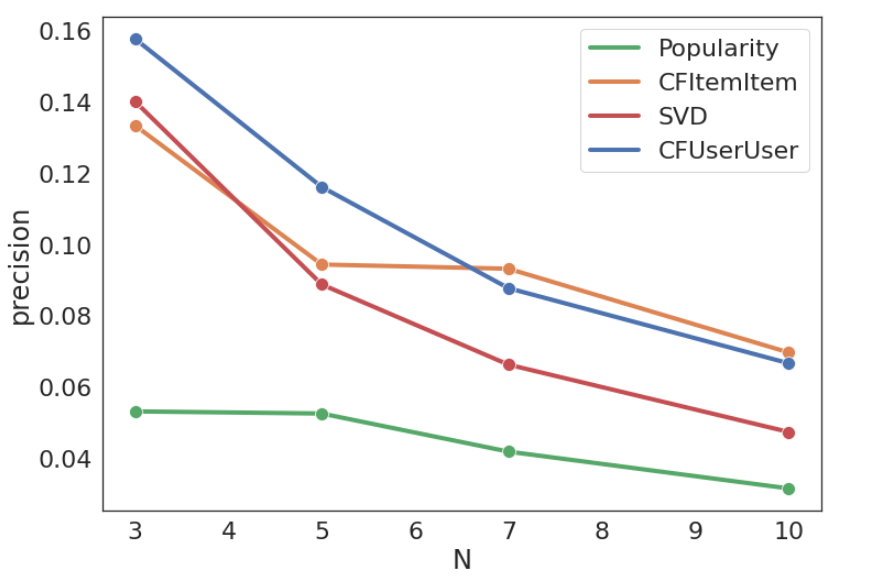
\includegraphics[width=7cm]{Figs/Presicion_N.png}
\caption{Precision results on offline data}
\label{fig:offline}
\end{figure}

 Fig ~\ref{fig:offline} shows results of the precision metric for
the 4 examined algorithms for different numbers of recommended projects. As can be seen from the figure,
collaborative filtering  Item-based and user-based are the best
algorithms and their performance is higher than popularity
and SVD for the data points measured. The popularity recommendation algorithm generated the lowest performance.

An interesting result is that for all algorithms, precision
drop drastically when recommending $n=5$
projects and continues to decrease for $n=7$ etc. The reason
for this decline is that in citizen science, volunteers generally
contribute to a low number of projects. For example, when
$n=5$, and the volunteer visited one of the new projects recommended by the algorithm,
its precision rate will be 1/5,
despite the fact that the algorithm was actually successful in
getting the user to try a new project.


Fig~\ref{fig:offlinehr} shows the hit rate of the different algorithms, defined as the percentage of instances in which users accessed at least one project that was recommended to them~\cite{wang2015recommendation}.
The hit rate for all algorithms rises consistently as the number of recommended projects increase.
The difference between user-based collaborative filtering and SVD was statistically significant for each $n$  using Mann-Whitney tests.
(for $n=3$, the default number of recommendations provided by the recommendation system in the online study, Mann-Whitney parameters were $U=376424.0, p < 0.05$)

\begin{figure}[t]
\centering
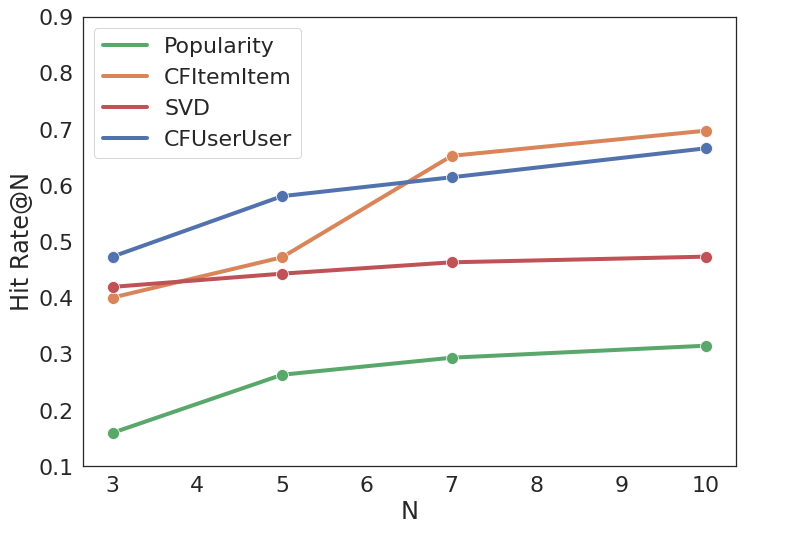
\includegraphics[width=7cm]{Figs/HitRate_N.png}
\caption{HitRate on offline data}
\label{fig:offlinehr}
\end{figure}
 \subsection{Online Study}

\begin{figure}[t]
\centering
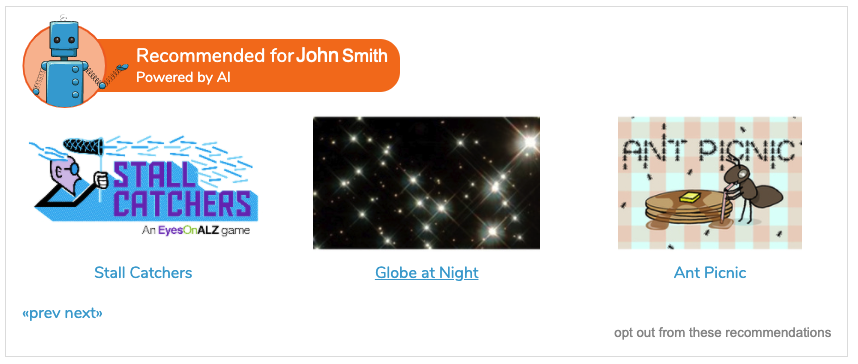
\includegraphics[width=8cm]{Figs/RecTool.png}
\caption{Screenshot of recommendation tool for user ``John Smith".}
\label{fig:fstat}
\end{figure}



The second part of the study  was an online experiment.   Users who logged on to SciStarter   starting on
 December 2\textsuperscript{nd}, 2019 were randomly assigned to one of  5 cohorts, each providing recommendations based on a different approach:
(1) Item-based collaborative filtering, (2) User-based collaborative filtering, (3)  Matrix factorization, (4) Most popular projects, (5) Promoted projects.   Projects in this category were manually determined by
SciStarter and often aligned with social initiatives and  current events.   Examples of such projects
%are GLOBE Observer Clouds\footnote{https://scistarter.org/globe-observer-clouds}, Stream Selfie \footnote{https://scistarter.org/stream-selfie} and TreeSnap \footnote{https://scistarter.org/treesnap}.
 %Another example is
 included FluNearYou (\url{flunearyou.org}), in which individuals report flu symptoms online,  and was one of the promoted
projects during the initial COVID-19 outbreak.
These projects are changed periodically  by the SciStarter administrators.

The recommendation tool  was active on SciStarter  for 3 months. Users who logged on during that time were randomly divided into cohorts, each receiving a recommendation
from a different algorithm. Each cohort had 42 or 43 users.
% Each user was given an option to opt-out from the experiment. Such users did not receive any recommendation and their data was not collected. In all of our experiments, none of the  users chose this option.
 The recommendations were embedded in the user's
dashboard in decreasing order of relevance, in sets of three,  from left to right. Users could scroll
to reveal more projects in decreasing or increasing order of relevance. Figure~\ref{fig:fstat} shows the   top three recommended projects for a target user.


All registered users  in SciStarter received notification via email about the study, stating that the  ``new SciStarter AI feature provides personalized recommended projects based on your activity and interests.'' A link to a blog post containing more
detailed explanations of recommendation algorithms and their role in the study was supplied.\footnote{\url{https://blog.scistarter.org/2019/09/smart-project-recommendations-on-scistarter/}} Additionally, the study privacy policy was explained and users were given the option to opt out of
receiving recommendations at any point in the experiment.  In practice, none of the participants selected the opt out option at any point in time.

%   We note that the personalized algorithms generated recommendations that were quite different from

%   We  illustrate that
% \begin{itemize}
% \item[\radiobutton] User A, who is assigned to User based collaborative filtering algorithm receives the recommended projects: [167,734,2992], which their popularity ranks are [11,16,19] respectively.
% \item[\radiobutton] User B, who is assigned to Item based collaborative filtering algorithm receives the recommended projects: [2992,83,114], which their popularity ranks are [19,12,25] respectively.
% \item[\radiobutton] User C, who is assigned to SVD algorithm receives the recommended projects: [890,671,87], which their popularity ranks are [3,1,6] respectively.
% \end{itemize}
% We can see that SVD recommends on less popular projects than other algorithms.


\begin{figure}[t]
     \centering
    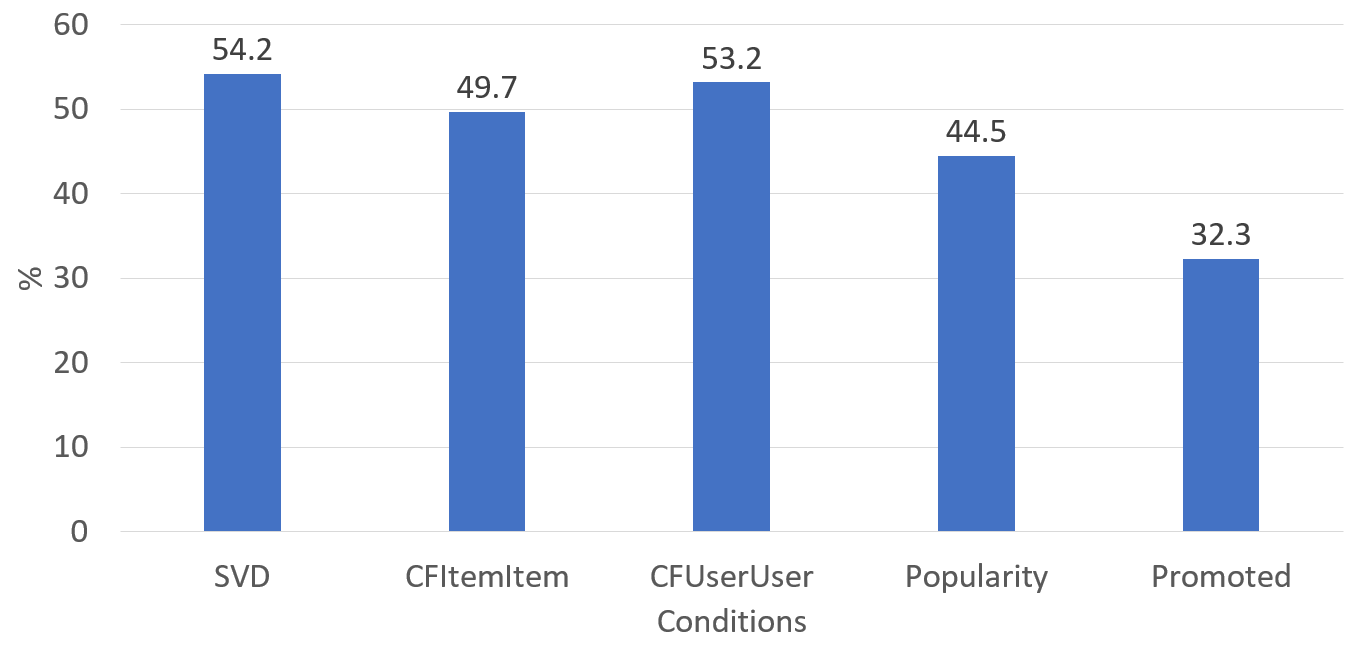
\includegraphics[width=8cm]{Figs/ctr.png}
        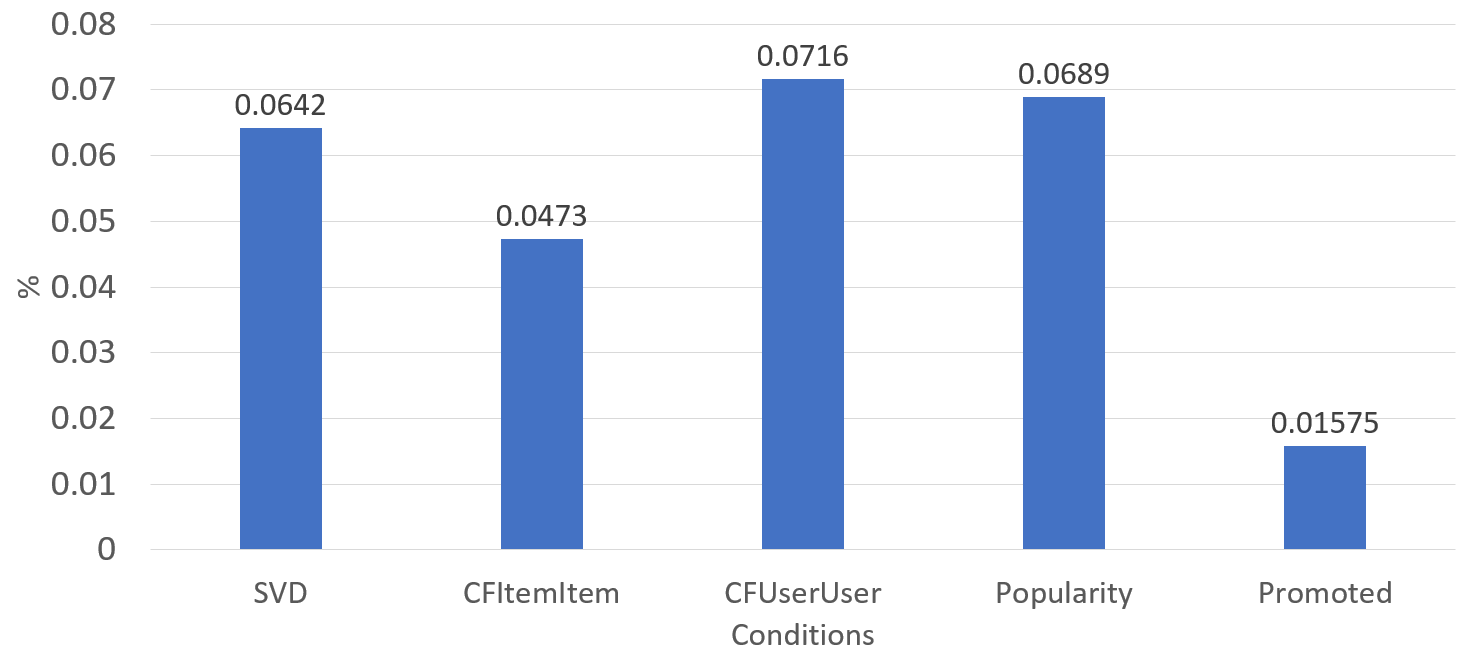
\includegraphics[width=8cm]{Figs/hit.png}
    \caption{Hit rate  (top) and Click through rate () and measures for  online study}
     \label{fig:hit}%
 \end{figure}

  Figure~\ref{fig:hit} (top) shows the  average hit rate (defined as the  percentage of instances in which users accessed at least one project that was recommended
  to them) and Figure~\ref{fig:hit} (bottom)  shows the  average click trough rate (defined as the ratio of recommended
  projects that the users accessed). As shown by the Figure, both  measures show a consistent trend, in which the
  user-based collaborative algorithms achieved the best performance, while the  promoted projects method achieving
  worse performance. Despite the trend, the differences between conditions were not statistically
  significant in the $p<0.05$ range. We attribute this  to measuring  clicks on recommended projects rather than  actual contributions
  which is the most important aspect for citizen science.

To address this gap we defined two new measures that consider the contributions made by participants
to projects, which constitutes the system utility as identified by Gunawardana and Shani~\cite{gunawardana2009survey}.
 The measures include the  average number of activities that users
carried out in recommended projects (RecE), and the average number of activities that users carried out in
non-recommended projects (NoRecE). Figure~\ref{fig:results} compares the different  algorithms according to these two measures. The results show that users assigned to the intelligent recommendation conditions  performed  significantly more activities in recommended projects than those assigned to the   popularity and promoted projects conditions.
Also, users in  the SVD algorithm performed  significantly less activities  in non-recommended projects than the popularity and promoted projects conditions.
% \kg{Naama please complete}. There is a clear trend  (though not statistically significant in the $p<0.05$ range) such
%that the SVD condition was most successful, followed by the item based CF and the user based CF algorithms.
These results
were statistically significant according to Mann-Whitney tests ($p<0.05$).
\begin{figure}[t]%
     \centering
    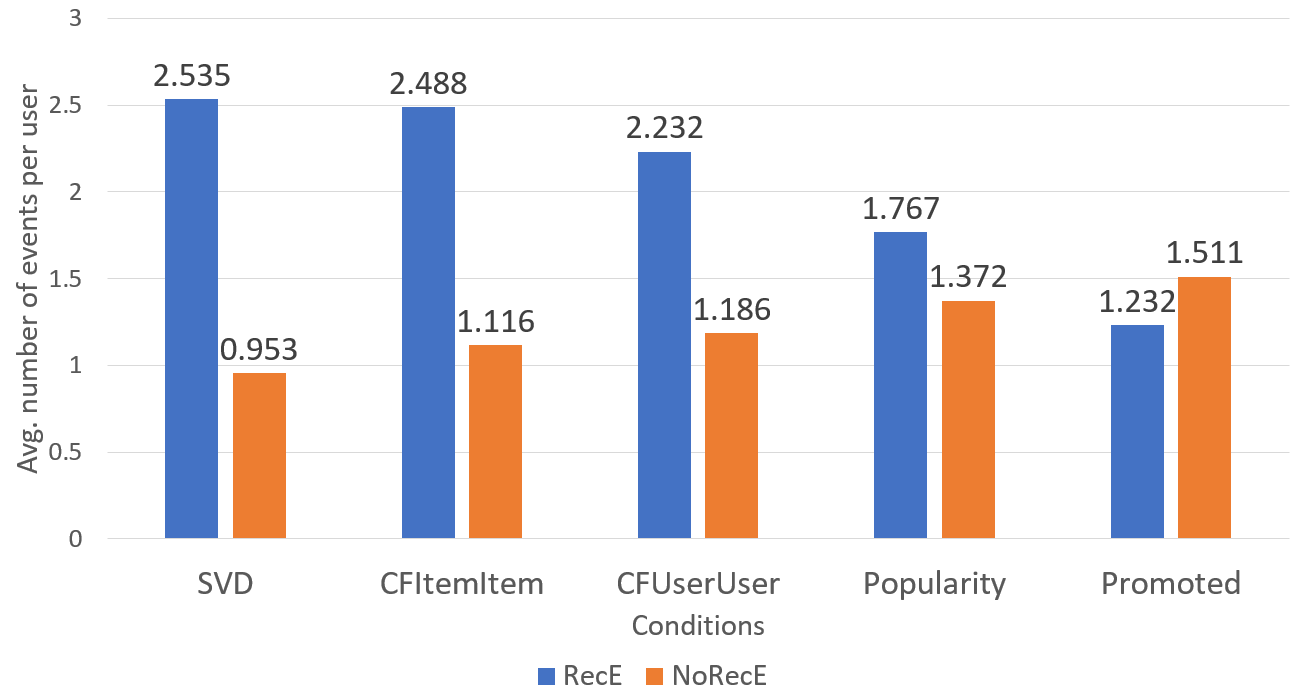
\includegraphics[width=8cm]{Figs/results1.png}
    \caption{Average activities on recommended projects (RecE), and on non-recommended
    projects (NoRecE) for each condition}
     \label{fig:results}%
 \end{figure}

 Lastly, we measure the average number of sessions  for users in the different conditions, where sessions are defined as a  continuous length of time in which the user is active in a project.
Figure~\ref{fig:results2} shows the average number of sessions for users in the different cohorts, including the number of sessions for the historical data used to train the algorithms, in which no recommendations
were provided.
The results show that users  receiving recommendations from the personalized algorithms
performed more sessions than the number of sessions in historical data. These results are statistically significant in the $p<0.05$ range using Mann-Whitney tests.
% \kg{Naama can you include details}
Although there is a clear trend that users in the $SVD$ condition achieved the highest number of sessions, these results were not significant in the $p<0.05$ range.




\begin{figure}[t]
     \centering
    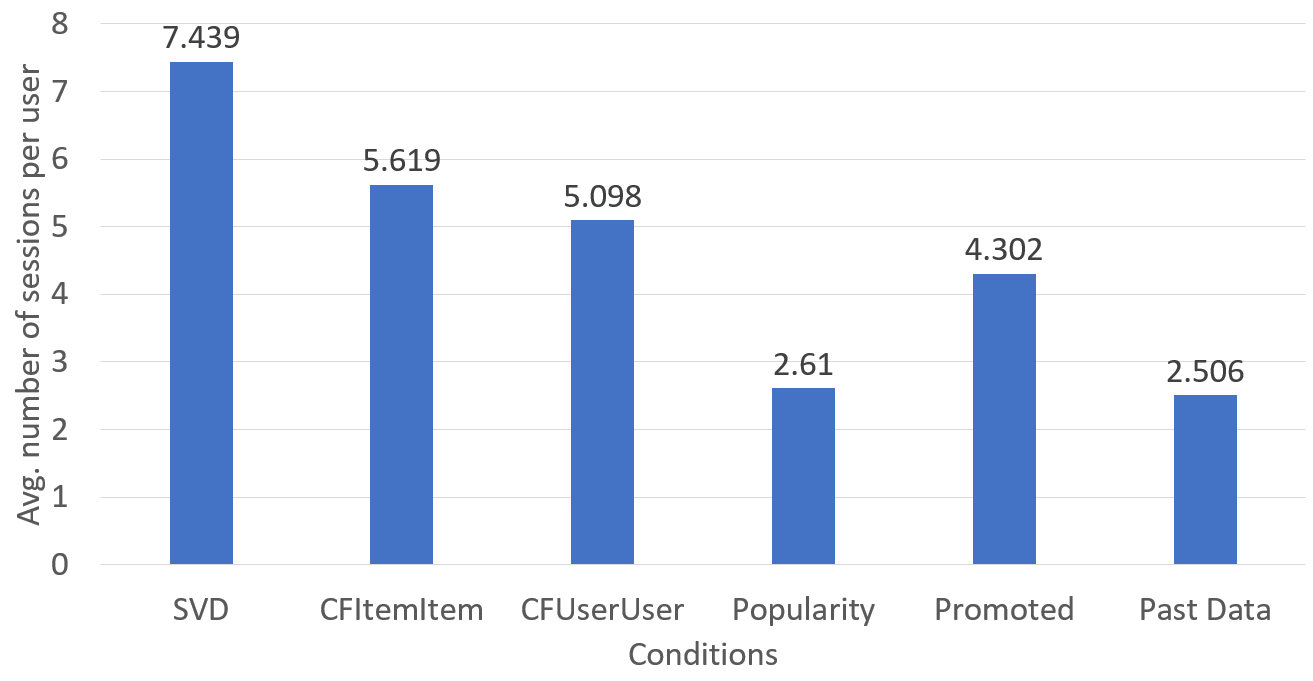
\includegraphics[width=8cm]{Figs/results2.png}
    \caption{Average number of sessions  for each condition}
     \label{fig:results2}%
 \end{figure}


To explain SVD's good performance in the online study, we first note that SVD is considered as a leading algorithm in the domain of recommendation systems \cite{sadek2012svd}.
Second, in our setting, SVD tended to generate recommendations that participants had not heard about before which seemed to resonate with many participants. As one participant remarked: ``I am more interested in projects I didn't know existed before".


Lastly, we note the obstacles we encountered when carrying out the study.
The first obstacle we encountered was the small number of relevant projects that could be recommended. Out of 3000 projects that SciStarter offers, we restricted ourselves to  153 affiliate projects which actively provide data of users' interactions.
Another obstacle was that we were constrained to a  subset of users who log on to the SciStarter platform
 and use it as a portal for contributing to  the project, rather than accessing the project
 directly.
Out of the 65,000 registered users of SciStarter, only a small percentage are logged in to both SciStarter and an affiliate project. As a result, we have relatively few users getting recommendations. In addition, some of SciStarter's projects are location-specific and can only be performed by users in the same physical location. (e.g collecting a water sample from a particular lake located in a particular city). Therefore, we kept track of users' location and restricted our recommendation system to be a location-based system, which recommends users with projects they are able to participate in.



\subsection {User Study}
In order to learn the users' opinion on the recommendations and their level of satisfaction, we conducted a survey with SciStarter's users. Our survey invitation was sent to all SciStarter community users. One hundred and thirty eight users have filled the survey, where each user was asked about the recommendations presented to them by the  algorithm they were assigned to. The survey included questions about users' overall satisfaction with the recommendation tool as well as questions about their pattern of behavior before and after the recommendations.


\begin{figure}
\centering
%\begin{picture}(220,100)
%\put(0,100){
\begin{small}
\end{small}
%\put(0,15)
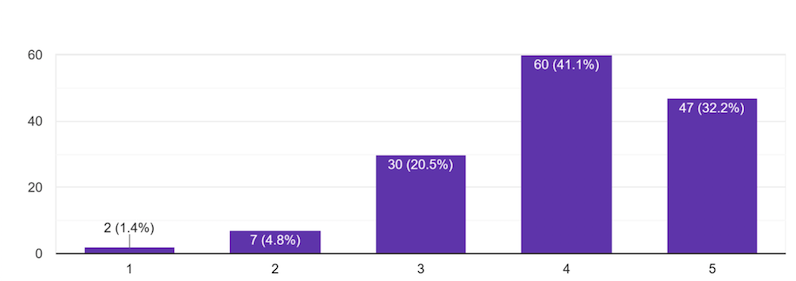
\includegraphics[width=7cm,height=2cm]{survrec.png}

How satisfied are you with the recommendation tool?

%\end{picture}
%\begin{picture}(220,130)
%\put(0,125){
\begin{small}\end{small}
%\put(0,10){
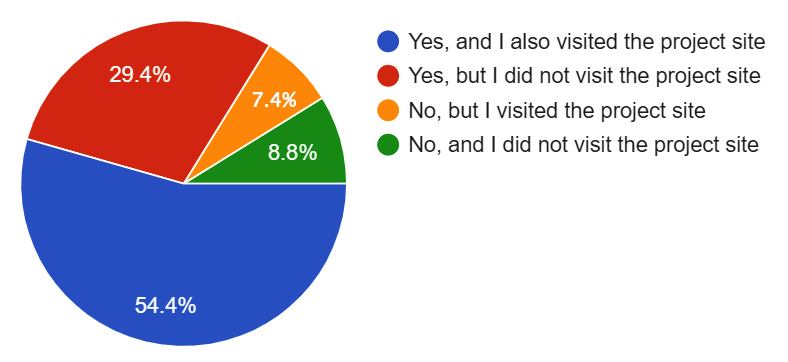
\includegraphics[width=7cm]{graph_survey1.png}
%\end{picture}

Did you click on one (or more) of the recommended projects?
    \caption{User satisfaction with recommendation tool (top) and User self report on clicking on recommended project (bottom)}
     \label{fig:userstudy}%
 \end{figure}
%, see \hyperref[fig:numperdec]{Figure \ref{fig:numperdec}}.
The majority of users (73.3\%; Responses 4 and 5 on a five-level Likert scale) were satisfied with the recommendation tool (Figure~\ref{fig:userstudy} top) and claimed that the recommendations matched their personal interests and goals. The majority of users (54\%) reported they have clicked on the recommendations and visited the project's site, while only 8.8\% of users did not click the recommendation nor visited the project site (Figure~\ref{fig:userstudy} bottom).


Interestingly, users who were not familiar with the recommended projects before, clicked more on the recommendations, as well as users who previously performed a contribution to a project.
Users who did not click on the recommendations can be divided into 3 main themes: (1) Users who didn't have the time ``right now" but planned to click the project in the future. (2) Users who felt that the recommendations were not suitable for their skills and materials: ``Seemed out of my league", ``I didn't have the materials to participate". This behaviour was also discussed in \cite{segal2015improving}, and was named ``classification anxiety". (3) Users who felt that the recommendations were not suitable for their interests: ``No interest in stall catchers", ``The photos and title didn't perfectly match what I am looking for".

The survey  result provide evidence for the positive impact of using the recommendation systems in  SciStarter. We note some additional comments by users: ``I am very impressed by the new Artificial Intelligence feature from SciStarter! Your AI feature shows me example projects that I didn't know before exist", and ``I like how personalized recommendations are made for citizen science users".



\section{Conclusion and Future Work}


This work reports on the use of recommendation algorithms to increase engagement of volunteers in citizen science, in which volunteers collaborate with researchers to perform scientific tasks.
These recommendation algorithms were deployed in   SciStarter, a portal with thousands of  projects,  and were evaluated in an online study involving hundreds of users who were informed about participating in a study involving AI based recommendation of new projects.
 We trained different recommendation algorithms using a combination of data including   users' behavior in SciStarter as well as their contributions to specific projects.  Our results show that using the new recommendation system  led people to contribute to  new projects that they had never tried before and  led to increased participation in SciStarter projects when compared to groups that were
recommended projects using non-personalized recommendation
approaches, and compared to behavior before recommendations.
%The AI-powered Recommendation system  has been fully deployed in  SciStarter.
 %when compared to  a  cohort group that did not receive recommendations.


 This project has transformed how SciStarter helps projects recruit and support participants and better respond to their needs. It was so successful in increasing engagement, that SciStarter has made the recommendation system a permanent feature of their site. This will help support deeper, sustained engagement to increase the collective intelligence capacity of projects and generate improved scientific, learning, and societal benefits.
%  The results of this research have been featured on the DiscoverMagazine.com~\footnote{\url{https://www.discovermagazine.com/technology/ai-powered-smart-project-recommendations-on-scistarter}}.
%

An important avenue for future work is to provide
users with explanations   to the recommendations in order to increase the system's reliability and user's satisfaction with it.  We also  plan to extend the recommendation system to include content based algorithms, and test its performance as compared to the existing algorithms. We believe that integrating content in citizen science domain (such as the project description, its location, age group etc.)  will enable us to
 %Even though users tend to participate in a variety of different projects, we want to be able to
 capture more intrinsic characteristic of the projects, such as required effort or type of task.

\section*{Acknowledgments}
Na'ama Dayan's work on this paper is equivalent to that of a co-author and is not recognized due to an oversight.
This work has received funding from the NESTA Collective Intelligence Grants 1.0 and from the European Union's Horizon 2020 WeNet research and innovation program under grant agreement No 823783. Thanks to Daniel Arbuckle  and Caroline Nickerson for their programming assistance and support.

% A crucial part of the study was to   quantitatively understand the relationships between SciStarter users and project activities (including project page views, bookmarks, joins, and contributions).
%  Among the 3,000+ projects registered on SciStarter, we narrowed our research to 80 SciStarter affiliate projects because these projects use APIs (see Participant API documentation: SciStarter.org/API) that report participants’ contributions back to SciStarter and back to the user. We limited the scope of research to SciStarter account holders (vs visitors to the site). Among the 70,000 SciStarter accounts, we further narrowed the study participants to those who engaged in at least two projects.

% % We use machine learning to explore the relationships between a user’s activities and profile on SciStarter, their referral source (where they came from before they reached SciStarter.org), their communities (Girl Scouts, schools, etc), and others who viewed, saved, joined or contributed to similar projects. Users were divided into cohorts. Then, once software detected patterns of engagement, algorithms were tested to select and display only three recommended projects to the select cohorts.

% Approximately 70,000 SciStarter users (including thousands of project leaders) have been informed about the  project and encouraged to login to SciStarter to test the new feature.



% In this work we have developed a recommendation system adapted to citizen science domain. Our recommendation system is based on users past activities, and provides personalized recommendations that are based on these activities. Our system was tested online and have proven its ability to increase users engagement to SciStarter.

% The use of the recommendation algorithm that we have developed has already  made a substantial impact on SciStarter.
% \hyperref[fig:example]{Figure \ref{fig:example}} demonstrates the increase in user participation in projects. Since experiment start date, there is a significant  increase in the number of users participation activities.
% %We can see that that our  outperforms all other algorithms, and particularly the baseline algorithm. Moreover, User based collaborative filtering and Popularity based algorithm, have also outperform the baseline algorithm, and thus succeeded to increase users engagement with the projects.

% In addition to the direct impact on SciStarter, our project demonstrated   a generalized approach for improving collective intelligence in citizen science by connecting users, data and AI. It showed  that  artificial intelligence can be used to guide citizen scientists through the SciStarter eco-system, matching them with projects selected by other users with similar characteristics, based on their profiles and logged activities. It directly increased  user engagement to enhance science learning and improve crowdsourced data quality because “becoming good requires practice” (Parrish et al. 2019)


% \begin{figure}%
%     \centering
%   %  \subfloat[]{
%     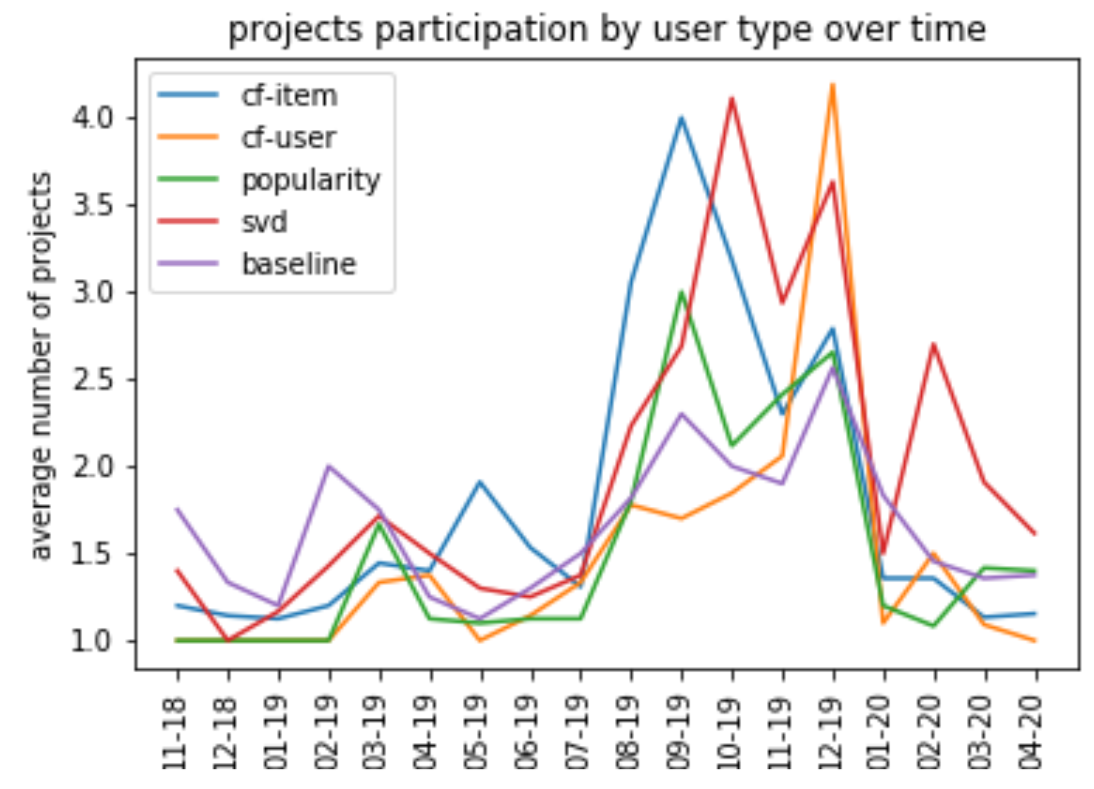
\includegraphics[width=7cm]{project_participation_by_algorithm (1).png} %
%   %  \qquad
%   % \subfloat[]{{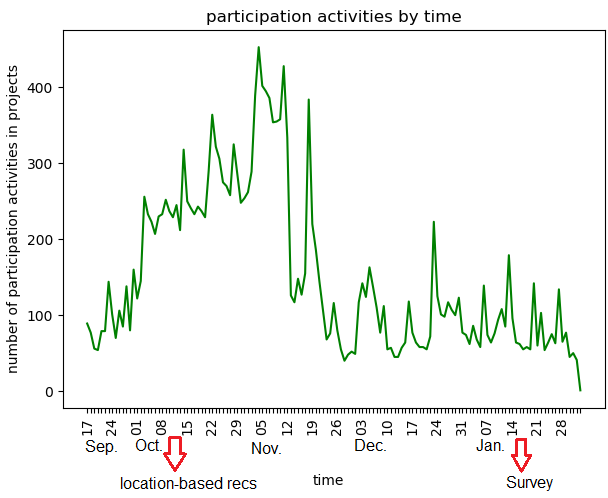
\includegraphics[width=5cm]{activity_experiment.png} }}%
%     \caption{Average number of participation activities in projects over time, where participation activities are any kind of participation in projects, such as data collection, classification, joining the project, etc.}%
%     \label{fig:example}%
% \end{figure}

% \begin{figure}%
%     \centering
%   %  \subfloat[]{
%     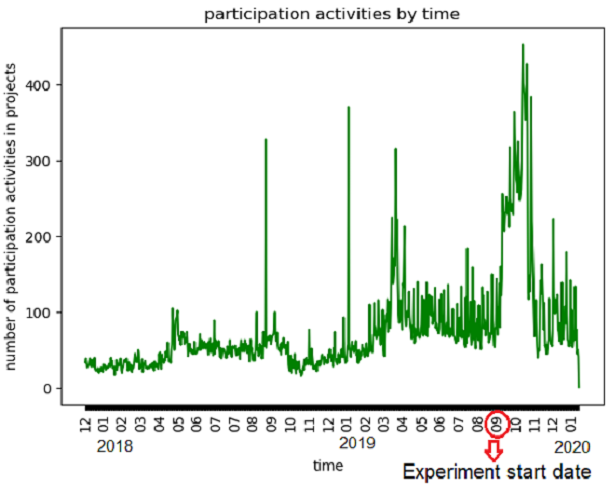
\includegraphics[width=7cm]{activity_count_by_time.png} %
%   %  \qquad
%   % \subfloat[]{{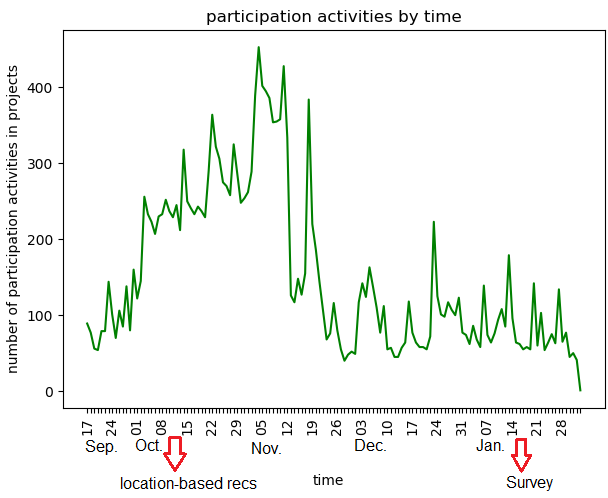
\includegraphics[width=5cm]{activity_experiment.png} }}%
%     \caption{Participation activities by time. The x axis describes the months between the beginning of year 2018 until beginning of year 2020. The y axis describes the total number of participation activities, where participation activities are any kind of participation in projects, such as data collection, classification, joining the project, etc.}%
%     \label{fig:example}%
% \end{figure}

% Our future work directly builds on the results of this NESTA project to  compare two badge pathways through SciStarter, a platform with 3,000 projects and 65,000 registered users: 1) assessment-based: recognition for completion of online module and assessments to measure acquired competencies and data contributions to projects; and 2) contribution-based: recognition strictly for participation. Badges for the first pathway, designed for public accreditation, will embed a list of skills and competencies that participants acquired, and begin to address social problems of educational attainment and unemployment. Projects will provide visible badge icons, and information about how to achieve the different badges.  We will base the study on 10 health research projects to help fill knowledge gaps about health inequalities.

% We will explore how badges can support sustained engagement in citizen science-which leads to better data contributions-by engaging stakeholders (U of Edinburgh, Arizona State U, SciStarter users, and Badgr, the only Mozilla authorized issuer) in the design and testing of two pathways using assessments, analytics, clickstreams and surveys to evaluate preferences and project data quality.

% Our hypotheses is that  1) badges will encourage sustained engagement benefitting a) participants through formalized recognition, and b) scientists through more and better data; 2) the optimal badge pathway will vary based on communities and motivations (e.g., assignments for college students vs volunteerism for senior citizens and library patrons).

\bibliographystyle{aaai21}
\clearpage
\bibliography{Article}

\end{document}
\appendix
\section{Appendix}
\subsection{Significance tests - number of activities}
A Mann-Whitney test was conducted to compare between each condition in the online experiment. Table~\ref{tab:significant_online} presents the results of the pairwise tests for the measures RecE and NoRecE that are significant.

\begin{table}[h]
\begin{center}
\begin{tabular}{|l|l|l|l|l|l|l|}
\hline
Condition1 & Condition2 & U     & n1 & n1 & DV     & Significant \\ \hline
CFUserUser & Popularity & 473.5 & 43 & 43 & RecE   & Yes         \\ \hline
CFUserUser & Baseline   & 406.0 & 43 & 43 & RecE   & Yes         \\ \hline
CFItemItem & Popularity & 458.5 & 43 & 43 & RecE   & Yes         \\ \hline
CFItemItem & Baseline   & 396.0 & 43 & 43 & RecE   & Yes         \\ \hline
SVD        & Popularity & 433.0 & 42 & 43 & RecE   & Yes         \\ \hline
SVD        & Baseline   & 371.5 & 42 & 43 & RecE   & Yes         \\ \hline
SVD        & CFItemItem   & 731.0 & 42 & 43 & RecE   & Yes         \\ \hline
SVD        & Baseline   & 729.0 & 42 & 43 & NoRecE & Yes         \\ \hline
% UserUserCF & Baseline   & 475.5 & 43 & 43 & ToolE  & Yes         \\ \hline
% ItemItemCF & Baseline   & 449.5 & 43 & 43 & ToolE  & Yes         \\ \hline
% SVD        & Popularity   & 713.0 & 42 & 43 & ToolE  & Yes         \\ \hline
% SVD        & Baseline   & 475.0 & 42 & 43 & ToolE  & Yes         \\ \hline
% Popularity & Baseline   & 552.5 & 43 & 43 & ToolE  & Yes         \\ \hline
\end{tabular}
\end{center}
\caption{Online Metrics - Mann Whitney significance test with p<0.05. DV=Dependent Variable}
\label{tab:significant_online}
\end{table}

\subsection{Significance tests - number of sessions}
A Mann-Whitney test was conducted to compare between each condition in the online experiment, including the historical data used to train the algorithms, called past-data. Table~\ref{tab:Significance2} presents the results of the pairwise tests that are significant.

\begin{table}[h]
\begin{center}
\begin{tabular}{|l|l|l|l|l|l|}
\hline
Condition1 & Condition2 & U      & n1                        & n2                         & Significant \\ \hline
CFUserUser & Past-Data  & 5898.0 & {\color[HTML]{222222} 43} & {\color[HTML]{222222} 557} & Yes         \\ \hline
CFItemItem & Past-Data  & 6502.0 & {\color[HTML]{222222} 43} & {\color[HTML]{222222} 557} & Yes         \\ \hline
SVD        & Past-Data  & 7284.0 & 42                        & 557                        & Yes         \\ \hline
Popularity & Past-Data  & 6683.5 & 43                        & 557                        & Yes         \\ \hline
Baseline   & Past-Data  & 6978.5 & 43                        & 557                        & Yes         \\ \hline
\end{tabular}
\end{center}
\caption{Number of sessions in SciStarter - Mann Whitney significance test with p<0.05}
\label{tab:Significance2}
\end{table}
